
\section{\ix Implementation}
\label{sec:impl}

\begin{table*}[t]
\centering
\begin{small}
\begin{tabular}{|l|l|l|}
\hline
\multicolumn{3}{|c|}{{\bf System Calls (batched)}} \\
\hline
connect &             cookie, dst\_IP, dst\_port		& Opens a connection\\
accept &              handle, cookie				& Accepts a connection\\
sendv &               handle, scatter\_gather\_array		& Transmits a scatter-gather array of data\\
recv\_done &          handle, bytes\_acked			& Advances the receive window and frees memory buffers\\
close &               handle					& Closes or rejects a connection\\
\hline  \hline
\multicolumn{3}{|c|}{{\bf Event Conditions}} \\
\hline
{\bf Type} &           {\bf Parameters}  &
{\bf Description}\\
knock  &               handle, src\_IP, src\_port		& A remotely initiated connection was opened \\
connected &            cookie, outcome				& A locally initiated connection finished opening \\
recv &                 cookie, mbuf\_ptr, mbuf\_len		& A message buffer was received \\
sent &                 cookie, bytes\_sent, window\_size	& A send completed and/or the window size changed \\
dead &                 cookie, reason				& A connection was terminated \\
\hline
\end{tabular}
\caption{\ix system calls and event conditions API. 
}
\label{tbl:api}
\end{small}
\end{table*}



We now describe the \ix prototype.  The current implementation uses
the VT-x features available on all x86-64
servers~\cite{DBLP:journals/computer/UhligNRSMABKLS05}. However, it can
be ported to any architecture with virtualization support, such as ARM
and Power.

% We start
% with an overview of the \ix kernel (\S\ref{sec:impl:kernel}), describe
% the environment surrounding \ix (\S\ref{sec:impl:env}), and how \ix is
% implemented as a coherency-free kernel (\S\ref{sec:impl:cohfree}).


%the benefits of having \ix run as a guest
%operating system (\S\ref{sec:impl:guest}), its native API at the
%kernel/user boundary (\S\ref{sec:impl:api}), the implementation of the
%networking stack (\S\ref{sec:impl:stack}), the implications on
%congestion management and flow control (\S\ref{sec:impl:net}), the
%benefits and consequences of coherence-free execution
%(\S\ref{sec:impl:cohfree}), and finally our approach to compatibility
%(\S\ref{sec:impl:libix}).

\subsection{Overview}
\label{sec:impl:overview}

Fig.~\ref{fig:cp-dp} presents the \ix architecture, including the
control plane, a number of dataplanes, and applications. The hardware
environment includes one or more multi-queue NICs with RSS support and
a multi-core server.

The \ix control plane consists of the full Linux kernel and
\texttt{IXCP}, a user-level program. The Linux kernel initializes PCIe
devices, such as the NICs, and provides the basic mechanisms for
resource allocation to the dataplanes, including cores, memory, and
network queues. Equally important, Linux provides system calls and
services that are necessary for compatibility with a wide range of
applications, such as file system and signal support. \texttt{IXCP}
monitors resource usage and dataplane performance and implements
resource allocation policies. The development of efficient allocation
policies involves understanding difficult tradeoffs between dataplane
performance, energy proportionality, and resource sharing between
co-located applications as their load varies over
time~\cite{Leverich:RHSU:2014,Lo:2014:TWE}. We leave the design of
such policies to future work and focus this paper on the \ix dataplane
architecture.

We run the Linux kernel in VMX root ring 0, the mode typically used to
run hypervisors in virtualized
systems~\cite{DBLP:journals/computer/UhligNRSMABKLS05}. We use the
Dune system within Linux to enable dataplanes to run as library-based
OSes in the VMX non-root ring 0, the mode typically used to run guest
kernels in virtualized systems~\cite{belay2012dune}. % \ana{Elaborate on
% role of Dune?}
Finally, applications run VMX non-root ring 3. This approach provides
dataplanes with direct access to hardware features, such as page
tables and exceptions, and provides full protection between the
control plane, dataplanes, and untrusted user code. Moreover,
dataplanes have direct passthrough access to  NICs.

 %\christos{should we explicitly say that most web-scale apps are
%  deployed without VMs so taking over VMX is not a problem?}\edb{not needed}

% \myparagraph{Separation and protection of control and data plane:}
% Each \ix instance and its applications runs as a distinct Dune process
% while control plane functions, including the control and monitoring of
% dataplane, is performed by scripts and daemons of the host
% environments.  This provides protection between control and
% dataplanes. Within each dataplane, \ix further protects itself from
% the untrusted application through virtual memory and by running it at
% userlevel.

% Section Move to the discussion session or future work
% \myparagraph{Elasticity policies:} In contrast to the mechanisms,
% which are generic, different policies can be envisioned to meet
% different use cases and optimization functions.  If neither energy
% proportionality or server consolidation is of any concern, the control
% plane can obviously launch a single dataplane instance configured with
% the maximal available physical resources.  In more realistic
% scenarios, the dataplane is ``right-sized'' to meet its service-level
% agreements with minimal resource allocations.  The control plane can
% further dynamically add or revoke CPUs from a dataplane instances,
% e.g., when the dataplane signals some sustained congestion or
% violation of its service-level agreements, or conversely when the
% allocated CPU resources are underutilized.


Each \ix dataplane supports a single, multithreaded
application. For instance, Fig.~\ref{fig:cp-dp} shows one dataplane
for a multi-threaded \texttt{memcached} server and another dataplane
for a multi-threaded \texttt{nginx} server. The control plane allocates
resources to each dataplane in a coarse-grained manner. Core allocation
is controlled through real-time priorities and \texttt{cpusets};
memory is allocated in large pages; each NIC hardware queue is
assigned to a single dataplane. This approach avoids the overheads and
unpredictability of fine-grained time multiplexing of resources between
demanding applications~\cite{Leverich:RHSU:2014}.

The \ix dataplane operates as a single address-space OS and supports
two thread types within the shared, user-level address space: (i)
\emph{elastic threads} which interact with the \ix dataplane to
initiate and consume network I/O and (ii) \emph{background threads}.
Both elastic and background threads can issue arbitrary POSIX system
calls that are intermediated and validated for security by the
dataplane before being forwarded to the Linux kernel.  Elastic
threads are expected to \emph{not} issue blocking calls because of the
adverse impact on network behavior and performance. Similarly, each
elastic thread makes exclusive use of a core or hyperthread allocated
to the dataplane in order to achieve high performance with predictable
latency. In contrast, multiple background threads may timeshare an
allocated hyperthread. For example, if an application were
allocated four hyperthreads, it could use all of them as elastic
threads to serve external requests or it could temporarily transition
to three elastic threads and use one background thread to execute
tasks such as garbage collection. When the control plane revokes or
allocates an additional hyperthread using a protocol similar to the
one used in Exokernel~\cite{DBLP:conf/sosp/EnglerKO95}, the dataplane
must adjust its number of elastic threads.

% We extended the Dune sandboxing mechanisms to support the initial load
% of multi-threaded applications into the userlevel address space, to
% launch both elastic and background threads.

\subsection{Dataplane API and Operation}
\label{sec:impl:kernel}

Elastic threads interact with the \ix dataplane through three
asynchronous, non-blocking mechanisms summarized in
Table~\ref{tbl:api}: they issue \emph{batched systems calls} to the
dataplane; they consume \emph{event conditions} generated by the
dataplane; and they have direct, but safe, access to message buffers
(\emph{mbuf}s) containing incoming payloads.  The latter  allows
for zero-copy access to incoming network traffic.  The application
can hold on to these message buffers until it asks the dataplane to
release them via the \texttt{recv\_done} batched system call.

Both batched system calls and event conditions are passed through
arrays of shared memory, managed by the user and the kernel
respectively.  We provide a regular system (\texttt{poll}) that serves
to yield control to the kernel and initiate a new run to completion
pass. As part of this process, the array of batched system call
requests is overwritten with the corresponding return codes and an
array of event conditions is populated. The handles defined in
Table~\ref{tbl:api} are kernel-level flow identifiers. Each handle is
associated with a cookie~\cite{han2012megapipe}, an opaque value
provided by the user at connection establishment to enable efficient
user-level state lookup. %without an additional table lookup.

\ix differs from POSIX sockets in that it directly exposes flow
control conditions to the application: the \texttt{sendv} system call
does not return the number of bytes buffered. Instead, it returns the
number of bytes that were accepted and sent by the TCP stack, as
constrained by correct TCP sliding window operation. Then, when the
bytes are acknowledged by the receiver, a \texttt{sent} event
condition informs the application that it is possible to send more
data. Thus, send window sizing policy is determined entirely by the
application.  By contrast, conventional OSes buffer send data beyond
raw TCP constraints and apply flow control policy inside the kernel
~\cite{dynamicwindow}.


% it alleviates the file descriptor number is lowest available
% requirement, which is not communative.  The reason for this
% requirement appears to be to allow user apps to easily make tables of
% meta-data pointers for each file descriptor.}

In addition to the low-level native \ix API in Table~\ref{tbl:api}, we
also built a user-level library that provides a compatible programming
model for legacy applications and significantly simplifies the
development of new applications. Our library provides a functionally
compatible interface to \texttt{libevent} and non-blocking POSIX
socket operations. It also includes new interfaces for zero copy read
and write operations that are more efficient, at the expense of
requiring changes to existing applications. 
%Our current implementation
%is missing certain features, such as support for timer events and
%high-level buffered I/O utilities.

\begin{figure}
%\hspace*{-0.25in}\centering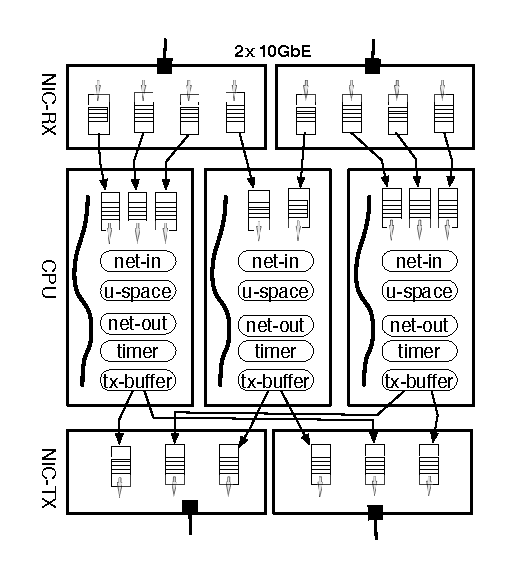
\includegraphics{figs/queues-cores.eps}
\centering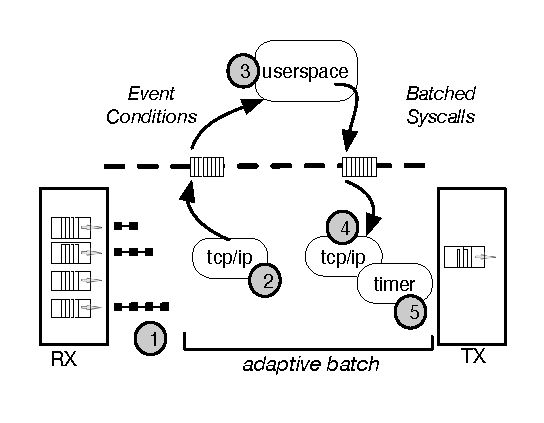
\includegraphics{figs/pipeline}
\caption{The IX pipeline.}
\label{fig:queues-cores}
\end{figure}

 

Fig.~\ref{fig:queues-cores} illustrates the run-to-completion
operation of elastic threads in the \ix dataplane. Each elastic thread
is associated with a specific set of receive queues from one or more
NICs. Each NIC uses RSS to implement flow-consistent hashing and
distribute incoming packets to queues. The queues are mapped in the
server's main memory and the NIC is given a set of buffer descriptors
that allow it to transfer incoming packets to memory using DMA\@.  The
elastic thread (1) polls the receive queues it is responsible for and
potentially posts fresh buffer descriptors to the NIC for use with
future incoming packets. The elastic thread (2) processes a bounded
number of packets through the TCP/IP networking stack, thereby
generating event conditions. Next, the elastic thread (3) passes
control to the user-space applications, which consumes all event
conditions. Assuming that the incoming packets include remote
requests, the application processes these requests and responds with a
batch of system calls. Upon return of control from user-space, the
elastic thread (4) processes all system calls, and in particular the
ones that direct outgoing TCP/IP traffic. It also (5) runs all kernel
timers in order to ensure compliant TCP behavior and (6) places
outgoing Ethernet frames in the NIC's descriptor rings for
transmission. Finally, it notifies the NIC to initiate a DMA transfer
for these frames by updating the transmit ring's tail register.  This
process repeats in a loop until there is no network activity. In this
case, we enter a quiescent state which involves either power-efficient
polling or yielding the hardware thread to the control plane.

% where we periodically poll the
% receive queues and potentially engage in power conservation states or
% yield to the control plane.

The \ix dataplane consists of 37K SLOC~\cite{url:sloccount}.  We
leveraged existing codebases in its development: 43\% is derived from
the DPDK variant of the Intel NIC device driver~\cite{intel:dpdk},
23\% from the lwIP TCP/IP stack~\cite{dunkels2001design}, and 16\%
from the Dune library.  All three code bases are highly modified for
\ix. The rest is approximately 7K SLOC of new code. We chose lwIP as a
starting point for TCP/IP processing because of its modularity and its
maturity as a RFC-compliant, feature-rich networking stack. We
implemented RFC-compliant support for UDP, ARP, and ICMP.
% It allows us to be RFC-compliant for TCP, UDP, ARP, and ICMP.
Since lwIP was optimized for memory efficiency in embedded
environments, we had to radically change its internal data structures
for multi-core scalability and fine-grain timer management. We did not
yet optimize the lwIP code for performance. Hence, there is room for
improvement in the results shown in \S\ref{sec:eval}.



\subsection{Multi-core Scalability}
\label{sec:impl:cohfree}

The \ix dataplane is optimized for multi-core scalability as elastic
threads operate in a synchronization and coherence free manner in the
common case. This is a stronger requirement than lock-free
synchronization, which requires expensive atomic instructions even
when a single thread uses a particular lock in the common
case~\cite{DBLP:conf/sosp/DavidGT13}.  This was made possible 
through a set of conscious design and implementation tradeoffs. 

First, the \ix API is commutative. Events are processed independently
on each elastic thread. Handles identify flows but cannot be exchanged
between elastic threads. There is no file descriptor namespace.
According to the commutativity rule, system call implementations can
only be coherence-free if the API itself is
commutative~\cite{DBLP:conf/sosp/ClementsKZMK13}.

Second, the API implementation is carefully optimized.  Each elastic
thread manages its own memory pools, hardware queues, event condition
array, and batched system call array. No synchronization is required
to access any of them. The implementation of event conditions and
batched system calls benefits directly from the explicit, cooperative
control flow transfers between \ix and the application by the elastic
thread.  Since there is no concurrent execution by producer and
consumer, event conditions and batched system calls are implemented
without synchronization primitives based on
atomics.

Third, the use of flow-consistent hashing at the NICs ensures that
each elastic thread operates on a disjoint subset of incoming TCP
flows. Hence, no synchronization or coherence occurs during the
processing of incoming requests for a server application. For client
applications with outbound connections, we need to ensure that the
reply is assigned to the same elastic thread that made the
request. Since we cannot reverse the Toeplitz hash used by RSS~\cite{url:rss}, we
simply probe the ephemeral port range to find a port number that
would lead to the desired behavior. Note that this implies that two
elastic threads in a client cannot share a flow to a server. % \edb{\sout{In
% \S\ref{sec:eval}, we show that \ix scales wells to hundreds of
% thousands of outgoing connections.}}
 
% ephemeral source port no longer form namespaces, which allows an \ix
% client to support millions of outgoing connections.


% \ix selects the source ephemeral port based on
% the requesting elastic thread. Since the Toeplitz hash function cannot
% be reversed, \ix simply probes the ephemeral range and computes the
% Toepliz hash until a match is found.  


\ix does have a small number of shared structures, including some that
require synchronization on updates.  For example, the ARP table is
shared by all elastic threads and is protected by RCU
locks~\cite{mckenney1998read}, Hence, the common case reads are
coherency-free but the rare updates are not.
%
\dm{Can you add a sentence about what constitutes a quiescent period
  for RCU garbage collection, given that this is a very non-Linux
  API?}

% Worth a paragraph break here, since reconfiguration is a big
% deal. -dm
\ix also requires
synchronization when the control plane reallocates resources between
dataplanes.  For instance, when a core is revoked from a dataplane,
the corresponding incoming queues must be assigned to another elastic
thread. Such events are rare because resource allocation happens in a
coarse-grain manner. Finally, the application code may include
inter-thread communication and synchronization. While using \ix does
not eliminate the need to develop scalable application code, it
ensures that there are no scaling bottlenecks in the system and
protocol processing code. 

%\subsection{Cooperative Flow Control}
\subsection{Security Model}
\label{sec:impl:coop}

%\adam{rename this section ``Security Design/Model'' ?}

The \ix API and implementation leads to a cooperative flow control
model between application code and the network-processing stack.  But
unlike user-level stacks that also expose networking behavior to user
code, \dm{Can you say something more specific than networking
  behavior?  Maybe something like ``unrestricted raw network
  access''?}  the \ix protection model makes few assumptions about
application behavior. A malicious or misbehaving application can only
hurt itself. It cannot corrupt the networking stack or affect other
applications.

The \ix dataplane and the application collaboratively manage
memory. To enable zero-copy operation, a buffer used for an incoming
packet is passed read-only to the application, enabling zero-copy
operation. Applications that hold on to message buffers for extensive
periods of time must bound their use of this shared resource.  In the
transmit direction, zero-copy operation implies that the application
must not modify outgoing data
% maintain outgoing data immutable
until reception is
acknowledged by the peer. % \edb{\sout{If there is recepient is not
    % operating fast enough or there is network congestion, the sender
    % will soon experience memory pressure as well.}}

Since elastic threads in \ix execute both the network stack and
application code, a long running application can block further network
processing for a set of queues. This behavior in no way affects other
applications or dataplanes. We use a timeout interrupt to detect
elastic threads that spend excessive time in user mode (e.g., in
excess of 10ms). We mark such applications as non-responsive and
notify the control
plane. %\edb{\sout{to potentially take resource allocation actions.}}

Note that all application code in \ix runs in user-mode, while the
dataplane code is in protected ring 0. Applications cannot access
dataplane memory, except for read-only message buffers.  No sequence
of batched system calls or other user-level actions can be used to
violate correct adherence to TCP and other network specifications.
Furthermore, the dataplane can be used to enforce network security
policies (e.g., iptables or Amazon Security
Groups~\cite{url:amazon-sg}) or to implement the network
virtualization functions typically done in a
hypervisor~\cite{nsdi:nsx}. Our security model is as strong as
conventional network stacks in commodity OSes and is missing from all
the recently proposed user-level networking stacks.

Our current implementation does not use an IOMMU due to their
performance overheads~\cite{iommu_overhead}. The \ix kernel is trusted
code that has access to descriptor rings with host-physical addresses.
This decision is not fundamental to our design and does not affect the
security model provided to applications. 

%Our current implementation does not yet utilize IOMMUs. As a result, a
%dataplane could potentially corrupt control plane memory through stray
%DMA operations. However, unlike user-level network stacks we do not
%strickly require IOMMU support, as untrusted application code is never
%s given direct access to NIC DMA engies. Rather, adding IOMMU support
%would improve security by creating a layer of in depth defense between
%dataplanes and control planes, possibly at the expensive of some
%performance overhead~\cite{iommu_overhead}.

\dm{This raised a couple of questions for me.  First, is the
  immutability of transmit buffers enforced by memory protection, or
  just by convention.  In other words, can you cause TCP segments to
  be sent with bad checksums or otherwise shoot yourself in the foot
  by writing to buffers in the send queue?  Second, why are message
  buffers read-only (or does this exclude the actual payload part).
  For example, if I'm implementing an HTTP proxy, can I make small
  modifications to a message buffer I just received and then
  retransmit it?  Or is the point that one would use scatter gather IO
  for such surgical edits?}
